\documentclass[12pt]{article} 
\usepackage[left=2cm, right=2cm, top=2cm, bottom=2cm]{geometry} 
\usepackage{graphicx}
\usepackage[pages=some]{background}
\usepackage{titling}
\usepackage{tabularx}
\usepackage{tikz}
\usepackage{textcase}
\usepackage{newtxtext}
\usepackage{enumitem}
\usepackage{fancyhdr}
\usepackage{multirow}
\usepackage{makecell}
\usepackage{amsmath}
\usepackage{amssymb}
\usepackage{subcaption}
\usepackage{float}
% \usepackage{figure}

\usetikzlibrary{positioning}

\pagestyle{fancy}
\fancyhf{} 
\renewcommand{\headrulewidth}{0pt} 
\rhead{\#1810009}

\begin{document}


  \subsection*{Experiment no: 3(a)}
  \subsubsection*{Name of the Experiment: Study and performance test of a submersible pump} 
  \vspace*{0.3cm}
  \subsection*{Objectives:}
  \begin{itemize}
    \item To study the working principle of a submersible pump.\item To determine the performance parameters of a submersible pump. 
    \item To plot the characteristic curve of a submersible pump and find its duty point. 
    \item To calculate the specific speed of a submersible pump. 
    
  \end{itemize}
  \subsection*{Apparatus:}
  \begin{enumerate}
    \item submersible Pump 
    \item Wattmeter 
    \item Flow meter 
    \item Manometer 
    \item Pressure Gauge 
    \item Stopwatch 
  \end{enumerate}  
  

  \subsection*{Schematic Diagram:}
  \begin{figure}[h]
    \begin{center}
      \includegraphics*[width=0.60\linewidth]{img/schematic.jpeg}
      \caption{Schematic diagram of a submersible pump test 
      }
    \end{center}
  \end{figure}
\pagebreak

\subsection*{Experimental measurement data:}
Datum Head of the PG (Pressure Gauge), $H_0$ = 2.21 m \\
PG calibration Equation: \\
Flowmeter calibration equation: $Y = 1.109 X - 2.201$ (LPM) \\

\subsubsection*{Data from the Experiment:}
\begin{center}
  \begin{tabularx}{\textwidth}{X*{4}{X}}
  \hline
  \multirow{3}{*}{\centering\makecell{No. of\\ Obs.}} & \multicolumn{2}{c}{\centering\makecell{Flow meter reading}} & \multirow{3}{*}{\centering\makecell{Pressure gauge\\ reading (psi)}} & \multirow{3}{*}{\centering\makecell{Input power, $P_{in}$\\Wattmeter reading\\(kW)}} \\ 
  \cline{2-3}
   & \multirow{2}{*}{\centering\makecell{Vol (lit)}} & \multirow{2}{*}{\centering\makecell{Time (s)}} & & \\
   & & & &
  \\
   \hline
  1 & 50 & 12.75 & 14 & 1.95 \\
  2 & 50 & 13.65 & 20 & 2.01 \\
  3 & 50 & 14.37 & 26 & 2.07 \\
  4 & 50 & 15.91 & 32 & 2.09 \\
  5 & 50 & 17.78 & 38 & 2.08 \\
  6 & 50 & 20.59 & 44 & 2.05\\
  7 & 50 & 25.41 & 50 & 2.03 \\
  8 & 30 & 20.69 & 56 & 1.96 \\
  9 & 30 & 36.31 & 62 & 1.86 \\
  10 & 5 & 123.78 & 68 & 1.70 \\ \hline 
  \end{tabularx}
  \end{center}

\vspace*{1cm}
\subsubsection*{Calculated Data:}
  \begin{center}
    \begin{tabularx}{\textwidth}{X*{6}{X}}
    \hline
    \multirow{2}{*}{\centering\makecell{No. of \\ obs.}} & \multicolumn{2}{c}{\centering\makecell{Flow rate / discharge, $Q$}} & \multirow{2}{*}{\centering\makecell{Head, $H$ \\m}} & \multirow{2}{*}{\centering\makecell{Input power,\\ $P_{in}$ (kW)}} & \multirow{2}{*}{\centering\makecell{Output power,\\ $P_{out}$ (kW)}} & \multirow{2}{*}{\centering\makecell{Overall effi., \\$\eta (\%)$}} \\
    \cline{2-3}
     & \centering\makecell{lit/min} & \centering\makecell{$m^3/s$} & & & & \\
    \hline
    1 & 258.74 & 4.31 $\times 10^{-3}$ & 12.06 & 1.95 & 0.51 & 26.15 \\
    2 & 241.54 & 4.03 $\times 10^{-3}$ & 16.275 & 2.01 & 0.643 & 31.99 \\
    3 & 229.31 & 3.82 $\times 10^{-3}$ & 20.494 & 2.07 & 0.768 & 37.10 \\
    4 & 206.91 & 3.45 $\times 10^{-3}$ & 24.71 & 2.09 & 0.836 & 40.00 \\
    5 & 184.92 & 3.08 $\times 10^{-3}$ & 28.93 & 2.08 & 0.874 & 42.01 \\
    6 & 159.38 & 2.66  $\times 10^{-3}$& 33.153 & 2.05 & 0.865 & 42.19 \\
    7 & 128.72 & 2.15 $\times 10^{-3}$ & 37.37 & 2.03 & 0.788 & 38.81 \\
    8 & 94.27 & 1.57 $\times 10^{-3}$ & 41.59 & 1.96 & 0.640 & 32.65 \\
    9 & 52.78 & 0.88 $\times 10^{-3}$ & 45.81 & 1.86 & 0.395 & 21.23 \\
    10 & 0.48 & 8.0 $\times 10^{-6}$ & 50.03 & 1.70 & $3.92\times 10^{-3}$ & 0.22 \\
    \hline
    \end{tabularx}
    \end{center}
\pagebreak

\subsection*{Sample Calculation:}
\textbf{For observation no.: 02}
\begin{enumerate}
  \item Discharge, $Q$ = Vol/Time = $\frac{50}{13.65}$ $lit/s$ = 3.663 $lit/s$ \\
  
  \hspace*{0.25\linewidth} = 219.78 lit/min 
  
  Actual discharge, $Q$ = (1.109 $\times$ 219.78 - 2.201) = 241.54 $lit/min$
  
  \hspace*{0.20\linewidth} = 4.03 $\times 10^{-3}$ $m^3/s$ 

  \item Head, 
  \begin{align*}
    H &= \frac{p}{\gamma} + H_0 \\
    &= \left(\frac{20 \times 6874.757}{9810} + 2.21 \right) \, m \text{ of Water}\\
    &= 16.275 \, m \text{ of Water}
  \end{align*}
  
  \item Input Power, $P_{in}$ = 2.01 kW 
  \item Output Power,
  \begin{align*}
    P_{out} &= \gamma Q H \\
    &=  9810 \times 4.03\times 10^{-3} \times 16.275 \, W \\
    &= 0.643 \, kW
  \end{align*}
  \item Overall Efficiency, 
  \begin{align*}
    \eta &= \frac{P_{out}}{P_{in}} \times 100\% \\
    &=\frac{0.643}{2.01} \times 100\%\\
    &=31.99\%
  \end{align*}
  
  \item Specific Speed (at best efficiency point), 
  
  \begin{align*}
    N_s &= \frac{N \sqrt{Q}}{H^{3/4}} \\
    &= \frac{2900 \times \sqrt{4.03\times 10^{-3}}}{(16.275)^{3/4}} \, rpm \\
    &= 22.72 \, rpm 
  \end{align*}
\end{enumerate}

\pagebreak
\begin{figure}[h]
  \begin{center}
    \includegraphics*[width=0.8\linewidth]{img/exp_3a.png}
  \end{center}
\end{figure}

\pagebreak
\subsection*{Discussion:}
From the charateristics curve, the operating point is found when:
\begin{align*}
  & Q = 0.00289\, m^3/s \\
  &\eta = 42.52\% \\
  &H = 31.01\, \text{m of Water} \\
  &P_{in} = 2.08\, kW \\
  &P_{out} = 0.88\, kW
\end{align*}


The $\eta$ vs $Q$ relationship in a submersible pump is characterized by an initial increase in efficiency followed by a decrease as the flow rate increases. This pattern arises due to multiple factors related to the pump's design and operational conditions. At low flow rates, the pump operates more efficiently due to reduced hydraulic losses and smoother internal fluid flow. However, as the flow rate increases beyond the optimal range, volumetric losses caused by leakage and internal recirculation start to rise, resulting in reduced efficiency. Mechanical losses, such as increased bearing friction and higher fluid forces, also contribute to decreased efficiency at higher flow rates. Additionally, a mismatch between the impeller design and the operating range can impact efficiency. The shape of the efficiency curve can vary based on the pump's design, impeller geometry, size, and type. \\


The point where the maximum efficiency is found is called "Best Efficiency Point" or "Operating Point". The operating point is the flow rate at which the pump operates most effectively, striking a balance between flow rate and head. It has a great significance in pump. Selecting the appropriate operating point ensures pump reliability and longevity. Deviating from the intended range can lead to wear and potential failures. The operating point impacts system performance and process optimization. By optimizing the operating point, costs associated with operation, maintenance, and energy consumption can be minimized.\\

Also in a submersible pump, the head decreases with an increase in flow rate due to the hydraulic and volumetric losses that occur within the pump. As the flow rate increases, there is greater resistance and turbulence within the pump, leading to higher losses and a decrease in the developed head.

\pagebreak

\subsection*{Experiment no: 3(b)}
\subsubsection*{Name of the Experiment:  Dismantling and assembling of a centrifugal pump} 
\vspace*{0.2cm}

\subsection*{Introduction:}
Centrifugal pumps are devices that are used to transport fluids by the conversion of rotational kinetic energy to the hydraulic energy of the fluid flow. The kinetic energy typically comes 
from an electric motor. Centrifugal pumps are used in more industrial applications than any other kind of pumps

\subsection*{Working Principle:}
Fluid enters the pump axially through the suction pipe to the eye of impeller (low pressure area) which rotates at high speed. As the impeller blades rotate, they transfer momentum to incoming fluid. The fluid accelerates radially outward, and a vacuum is created at the impellers eye that continuously draws more fluid into the pump. As the fluid's velocity increases its kinetic energy increases. Fluid of high kinetic energy is centrifugally forced out of the impeller area and enters the volute. In the volute, the fluid flows through a continuously increasing cross sectional area, where the kinetic energy is converted into fluid pressure according to Bernoulli's principle. The main parts of a centrifugal pump include the suction pipe, impeller, volute casing, shaft, packing seals, bearing etc. The impeller may be open, semi open, or closed 
type depending on the fluid to be handled. 


\subsection*{Activities:}
1. Dismantle a centrifugal pump using the tools provided. \\
2. Identify and observe each of the components. \\
3. Take photographs of various components and attach them with the report. \\
4. Study the components and energy flow sequence. \\
5. Assemble all components to form the pump again. \\

\begin{figure}[H]
  \begin{center}
    \includegraphics*[width=0.9\linewidth]{img/cetrifugal_pump.jpeg}
  \end{center}
\end{figure}

\subsection*{Pump Component Sequence:}
\vspace*{0.5cm}
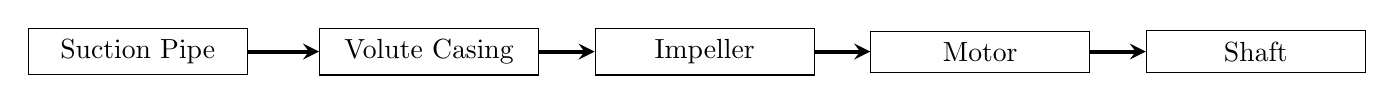
\begin{tikzpicture}[node distance=2cm, every node/.style={rectangle, draw, align=center, text width=2.5cm, inner sep=4pt}]
  \node (start) {Suction Pipe};
  \node (node1) [right of=start, node distance=3.7cm] {Volute Casing};
  \node (node2) [right of=node1, node distance=3.5cm] {Impeller};
  \node (node3) [right of=node2, node distance=3.5cm] {Motor};
  \node (end) [right of=node3, node distance=3.5cm] {Shaft};
  
  \draw[->, >=stealth, line width=1.5pt] (start) -- (node1);
  \draw[->, >=stealth, line width=1.5pt] (node1) -- (node2);
  \draw[->, >=stealth, line width=1.5pt] (node2) -- (node3);
  \draw[->, >=stealth, line width=1.5pt] (node3) -- (end);
\end{tikzpicture}

\subsection*{Energy Conversion Sequence:}
\vspace*{0.5cm}
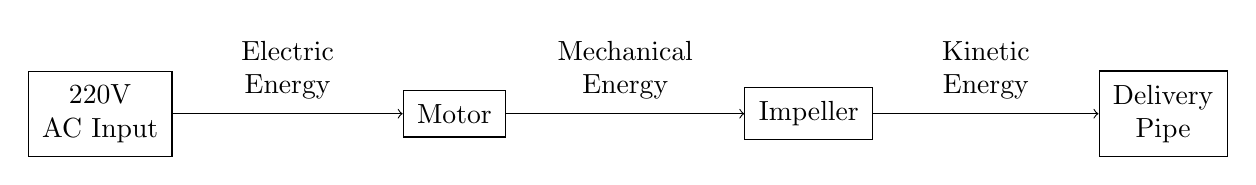
\begin{tikzpicture}[node distance=4.5cm, every node/.style={rectangle, align=center, inner sep=5pt}]
  \node[draw] (start) {220V \\AC Input};
  \node[draw, right of=start] (process1) {Motor};
  \node[draw, right of=process1] (process2) {Impeller};
  \node[draw, right of=process2] (end) {Delivery\\Pipe};
  
  \draw[->] (start) -- node[above]{Electric\\Energy} (process1);
  \draw[->] (process1) -- node[above]{Mechanical\\Energy} (process2);
  \draw[->] (process2) -- node[above]{Kinetic\\Energy} (end);
\end{tikzpicture}
\vspace*{0.5cm}

\subsection*{Questions \& Answers:}

\textbf{1. Where are the gaskets placed??}\\
\textbf{Ans:} Gaskets are positioned in centrifugal pumps to create a seal between two surfaces, ensuring that fluids do not leak. They are commonly employed in areas like pump casings, flanges, and connections.

\vspace*{0.3cm}\hspace*{-0.035\linewidth}
\textbf{2. Why gland packing seals are used?}\\
\textbf{Ans:} Gland packing seals are used in centrifugal pumps for several reasons. They provide a reliable sealing solution that helps prevent leakage along the pump shaft. Gland packing seals can accommodate shaft movement and vibration, making them suitable for dynamic applications. They also allow for adjustment and tightening as needed to maintain the desired level of sealing effectiveness.

\pagebreak

\begin{figure}
  \centering

  \begin{subfigure}{0.3\textwidth}
      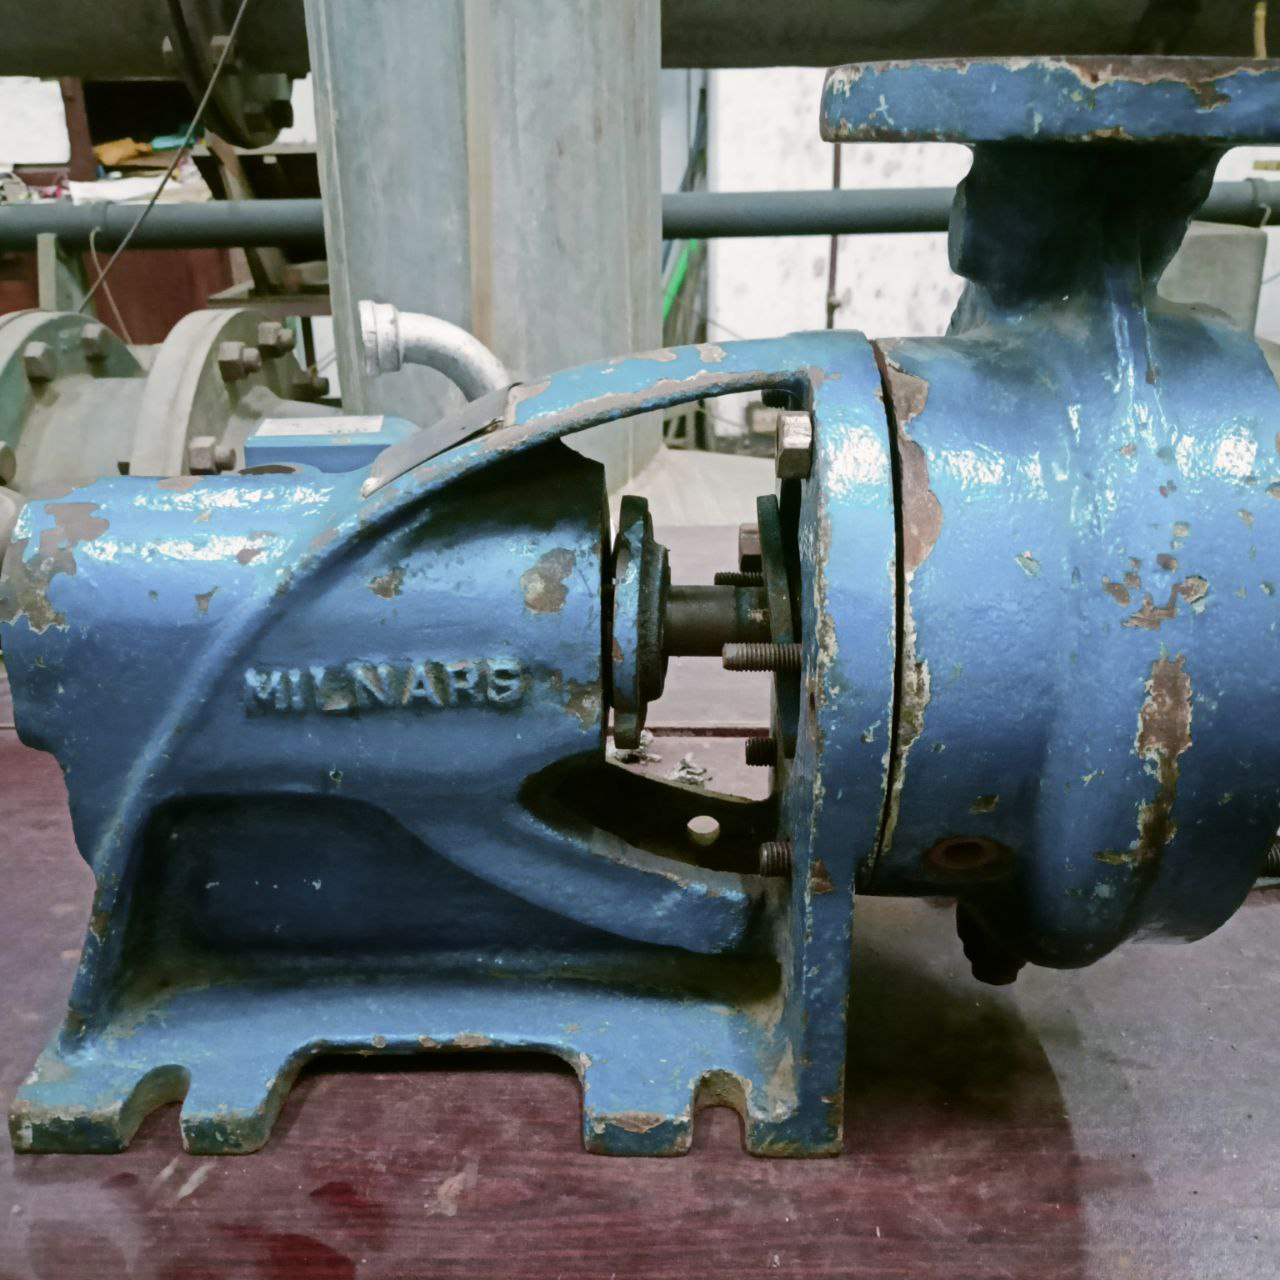
\includegraphics[width=\linewidth]{img/p_01.jpg}
      \caption{Pump}  
  \end{subfigure}
  \hfill
  \begin{subfigure}{0.3\textwidth}
      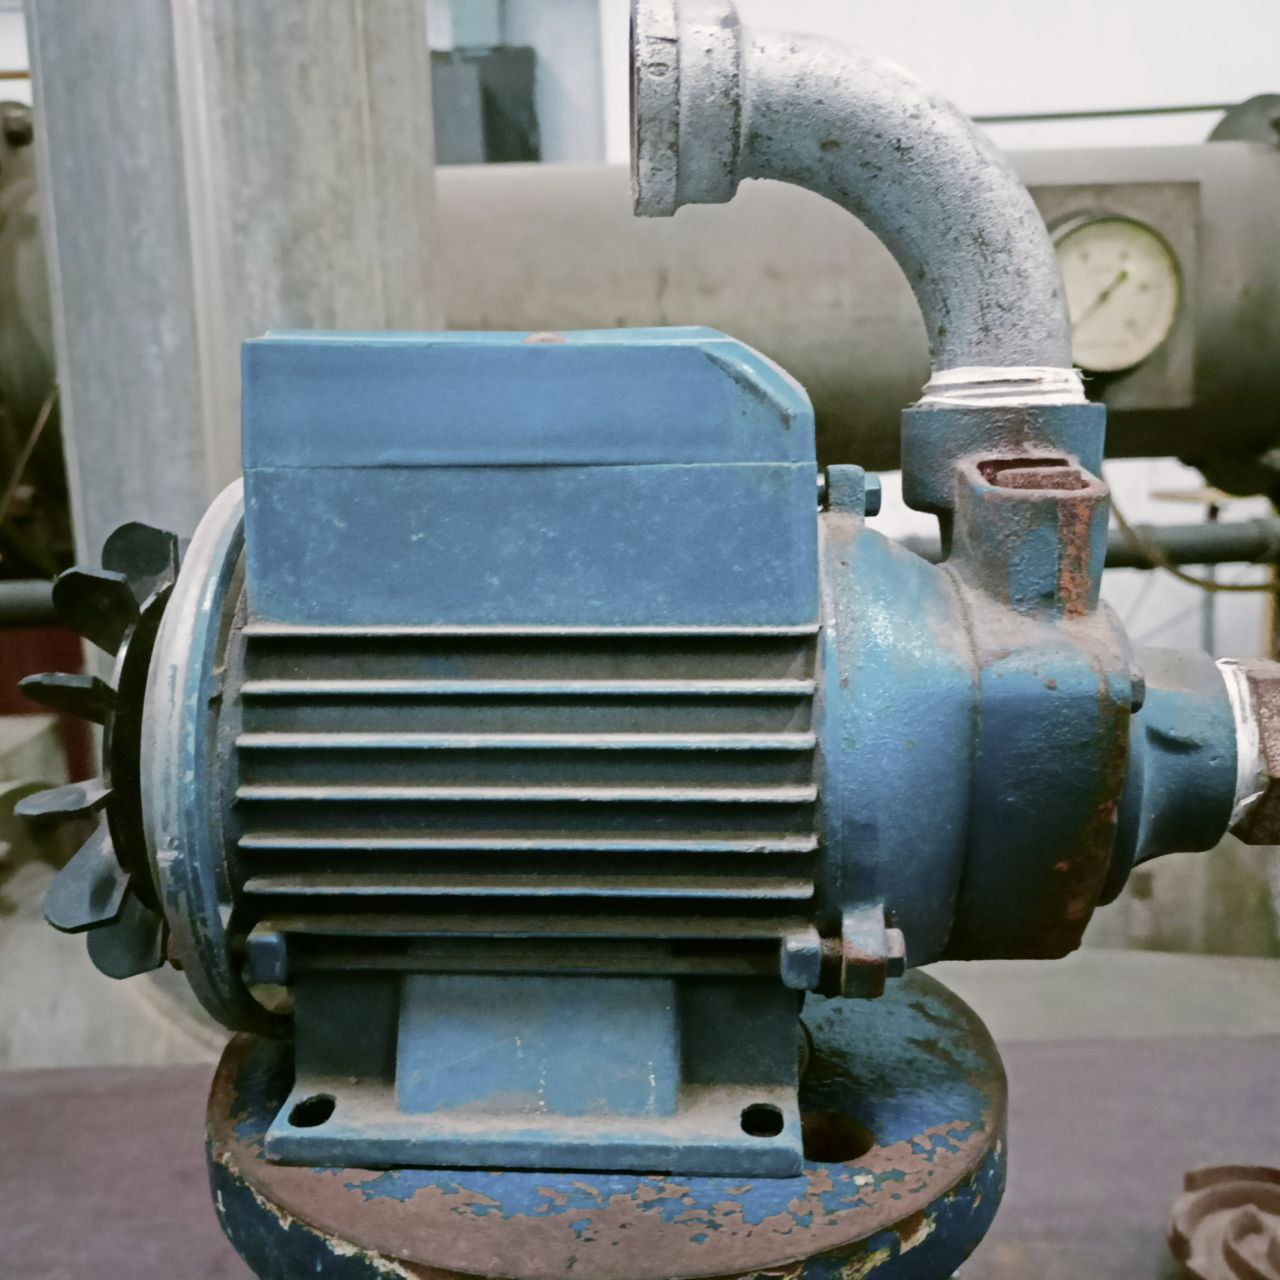
\includegraphics[width=\linewidth]{img/p_02.jpg}
      \caption{Motor}
  \end{subfigure}
  \hfill
  \begin{subfigure}{0.3\textwidth}
      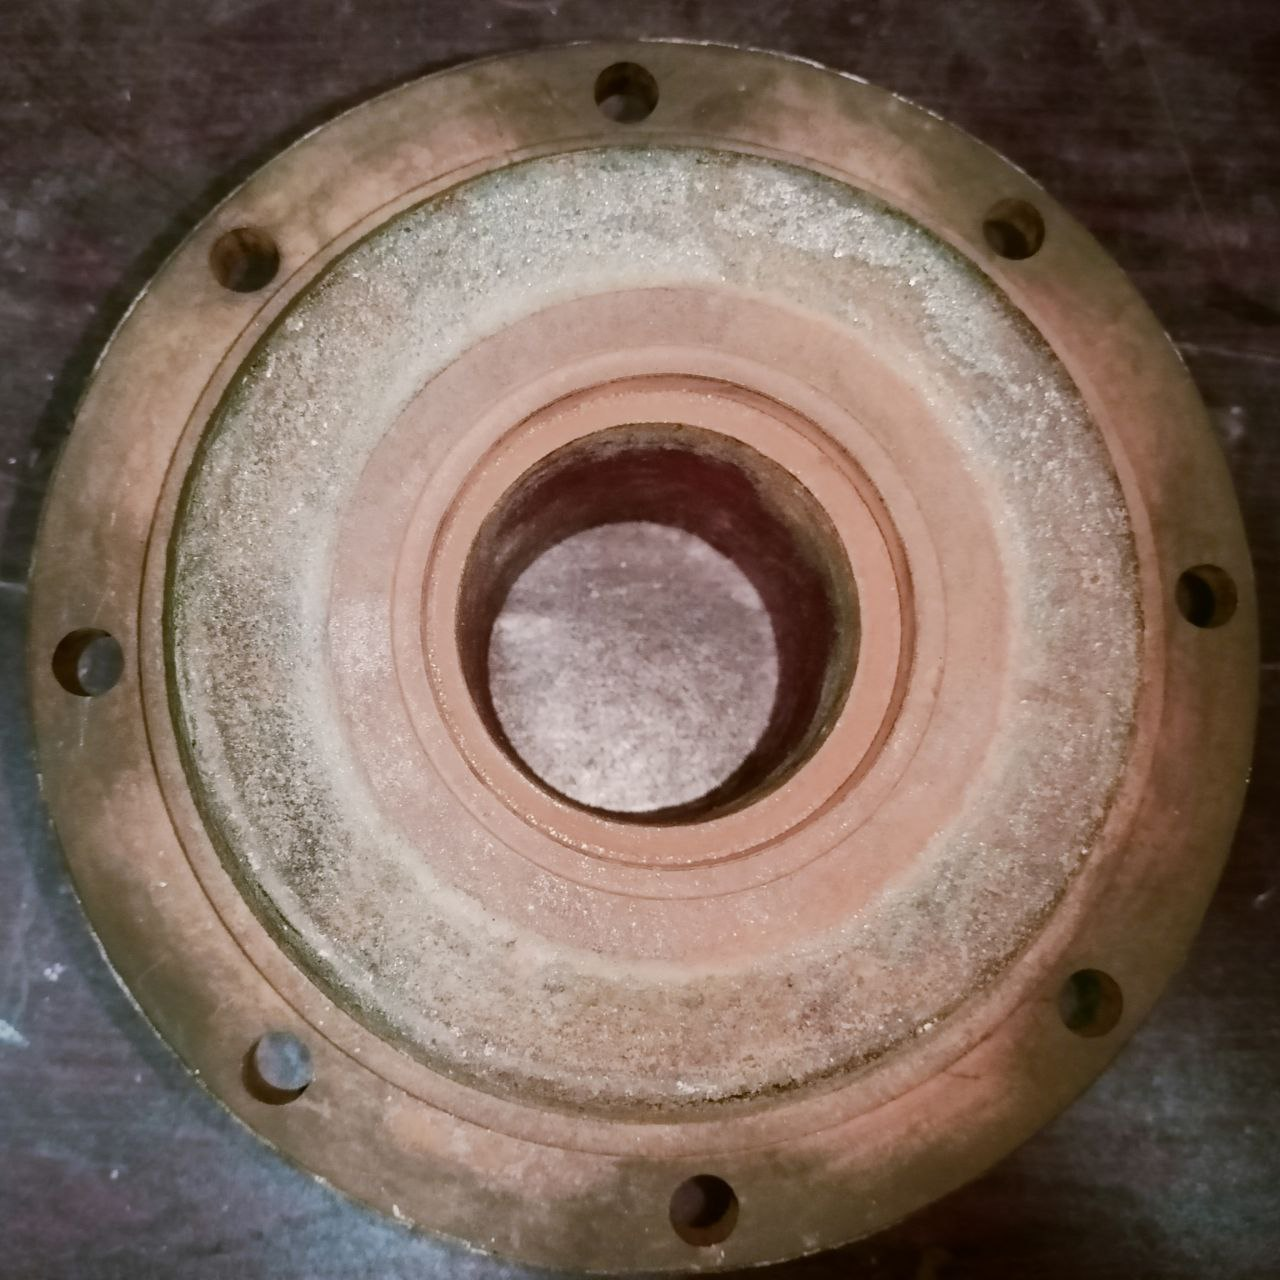
\includegraphics[width=\linewidth]{img/p_03.jpg}
      \caption{Suction Pipe}
  \end{subfigure}

  \vspace{0.5cm}

  \begin{subfigure}{0.3\textwidth}
      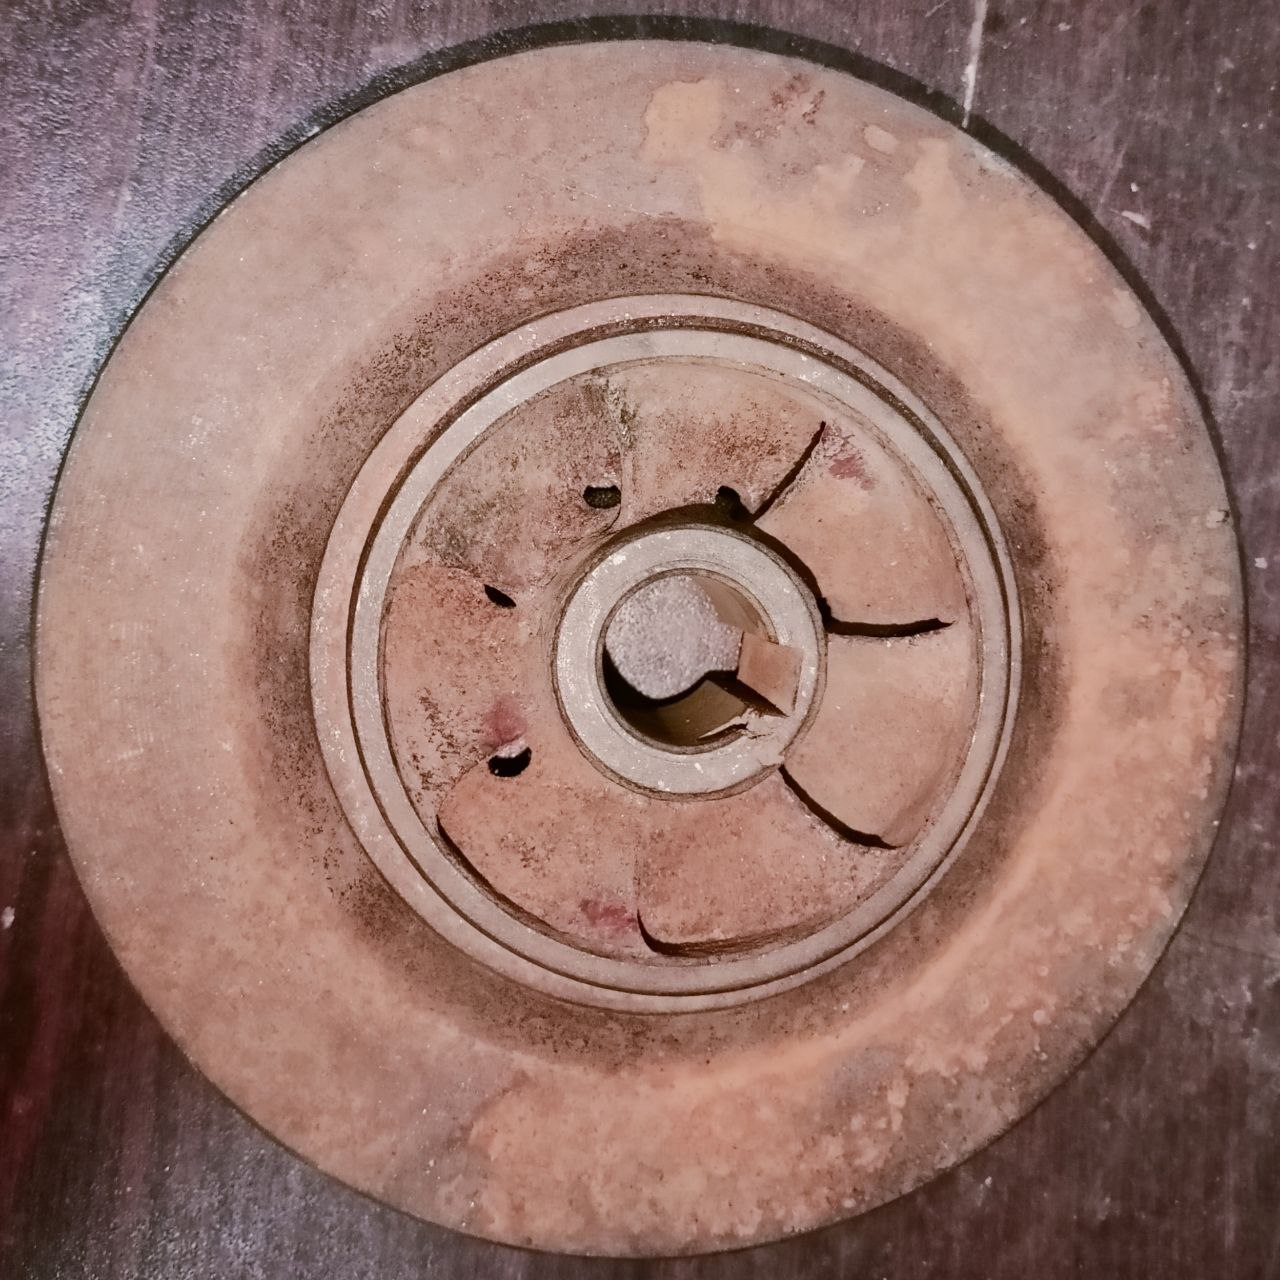
\includegraphics[width=\linewidth]{img/p_04.jpg}
      \caption{Impeller}
  \end{subfigure}
  \hfill
  \begin{subfigure}{0.3\textwidth}
      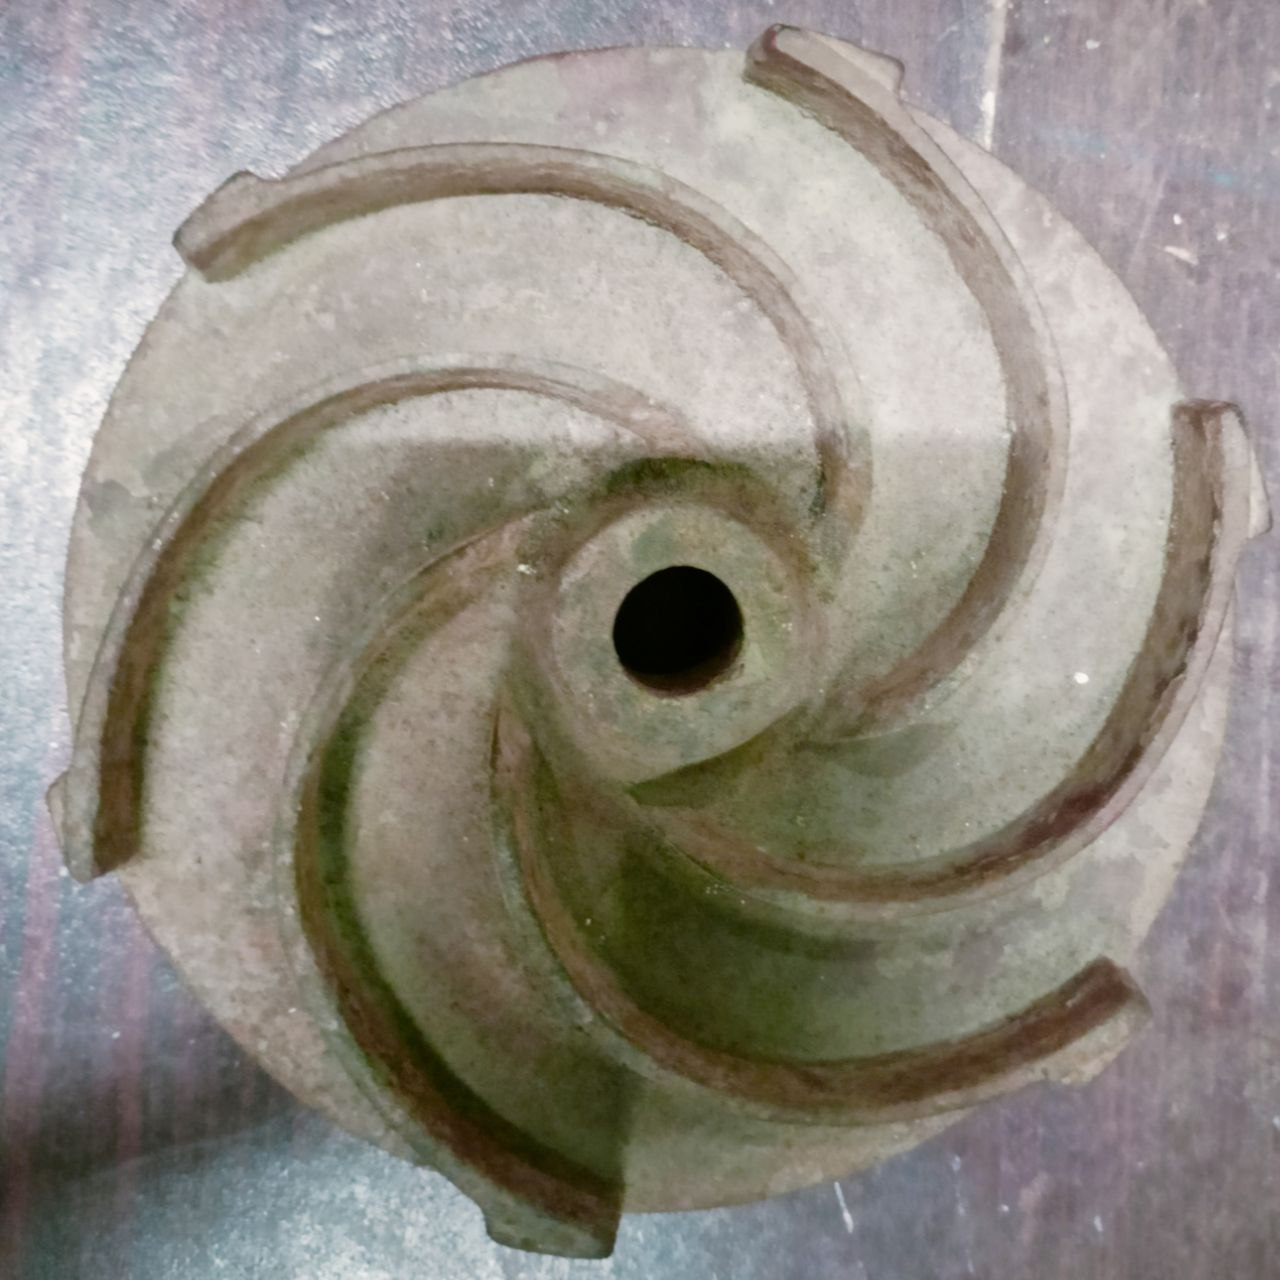
\includegraphics[width=\linewidth]{img/p_05.jpg}
      \caption{Vane/Diffuser}
  \end{subfigure}
  \hfill
  \begin{subfigure}{0.3\textwidth}
      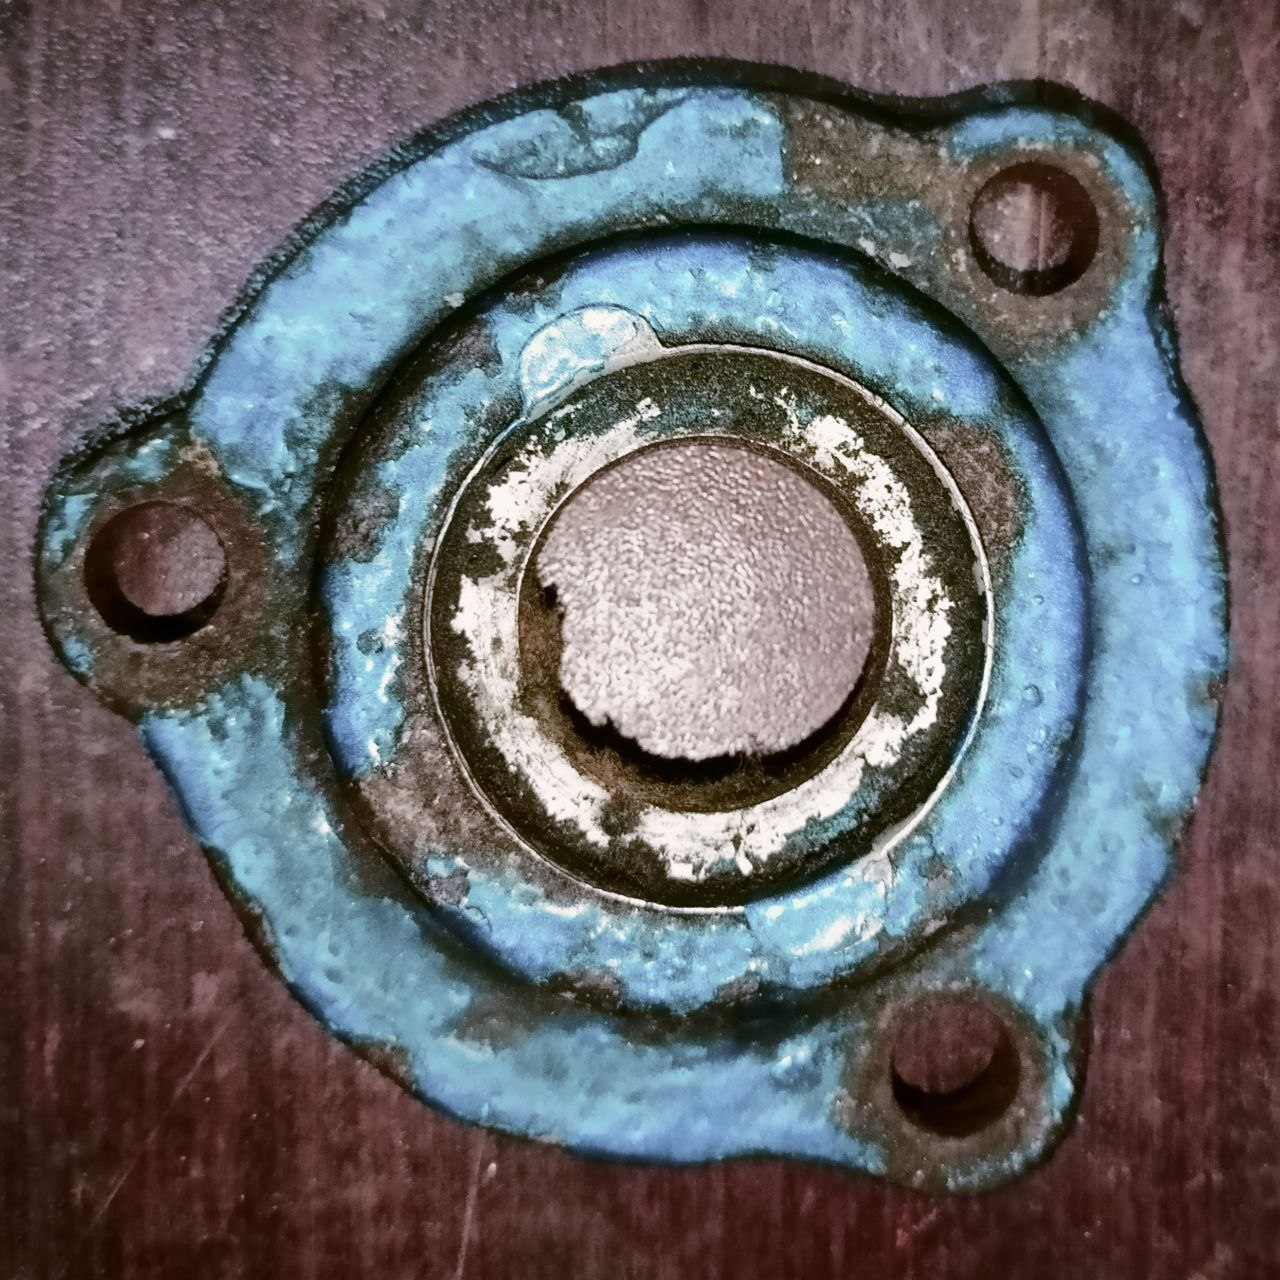
\includegraphics[width=\linewidth]{img/p_06.jpg}
      \caption{Flange}
  \end{subfigure}

  \vspace{0.5cm}

  \begin{subfigure}{0.3\textwidth}
      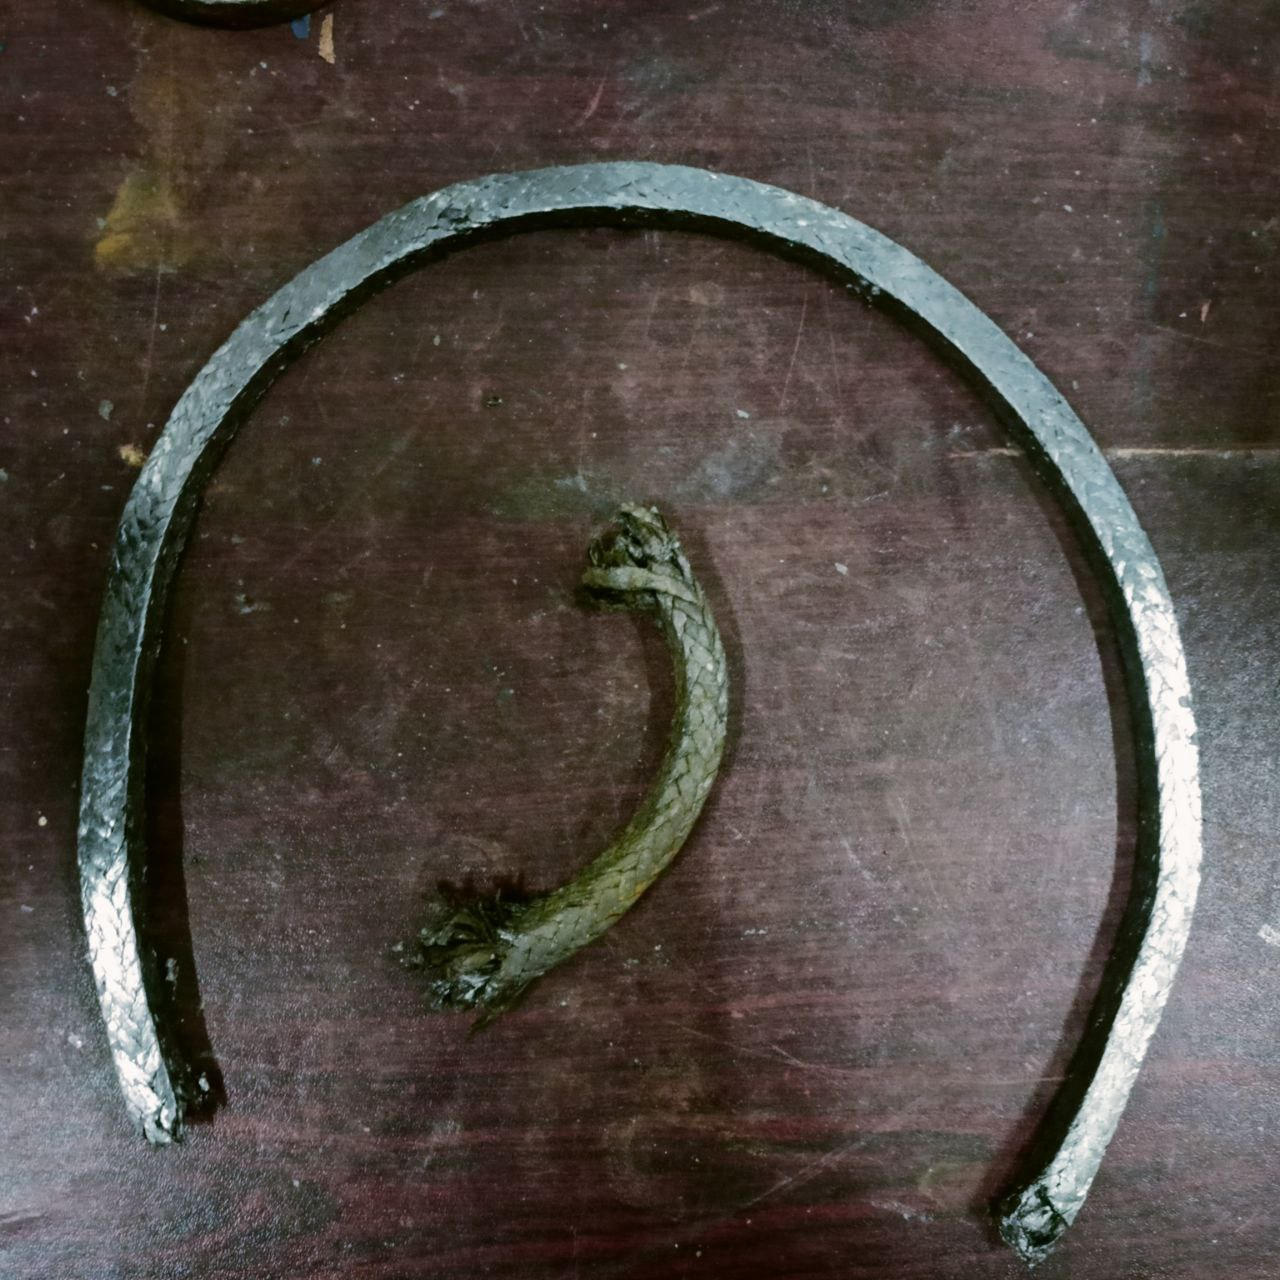
\includegraphics[width=\linewidth]{img/p_07.jpg}
      \caption{Asbestos rope (Gland Packing)}
  \end{subfigure}
  \hfill
  \begin{subfigure}{0.3\textwidth}
      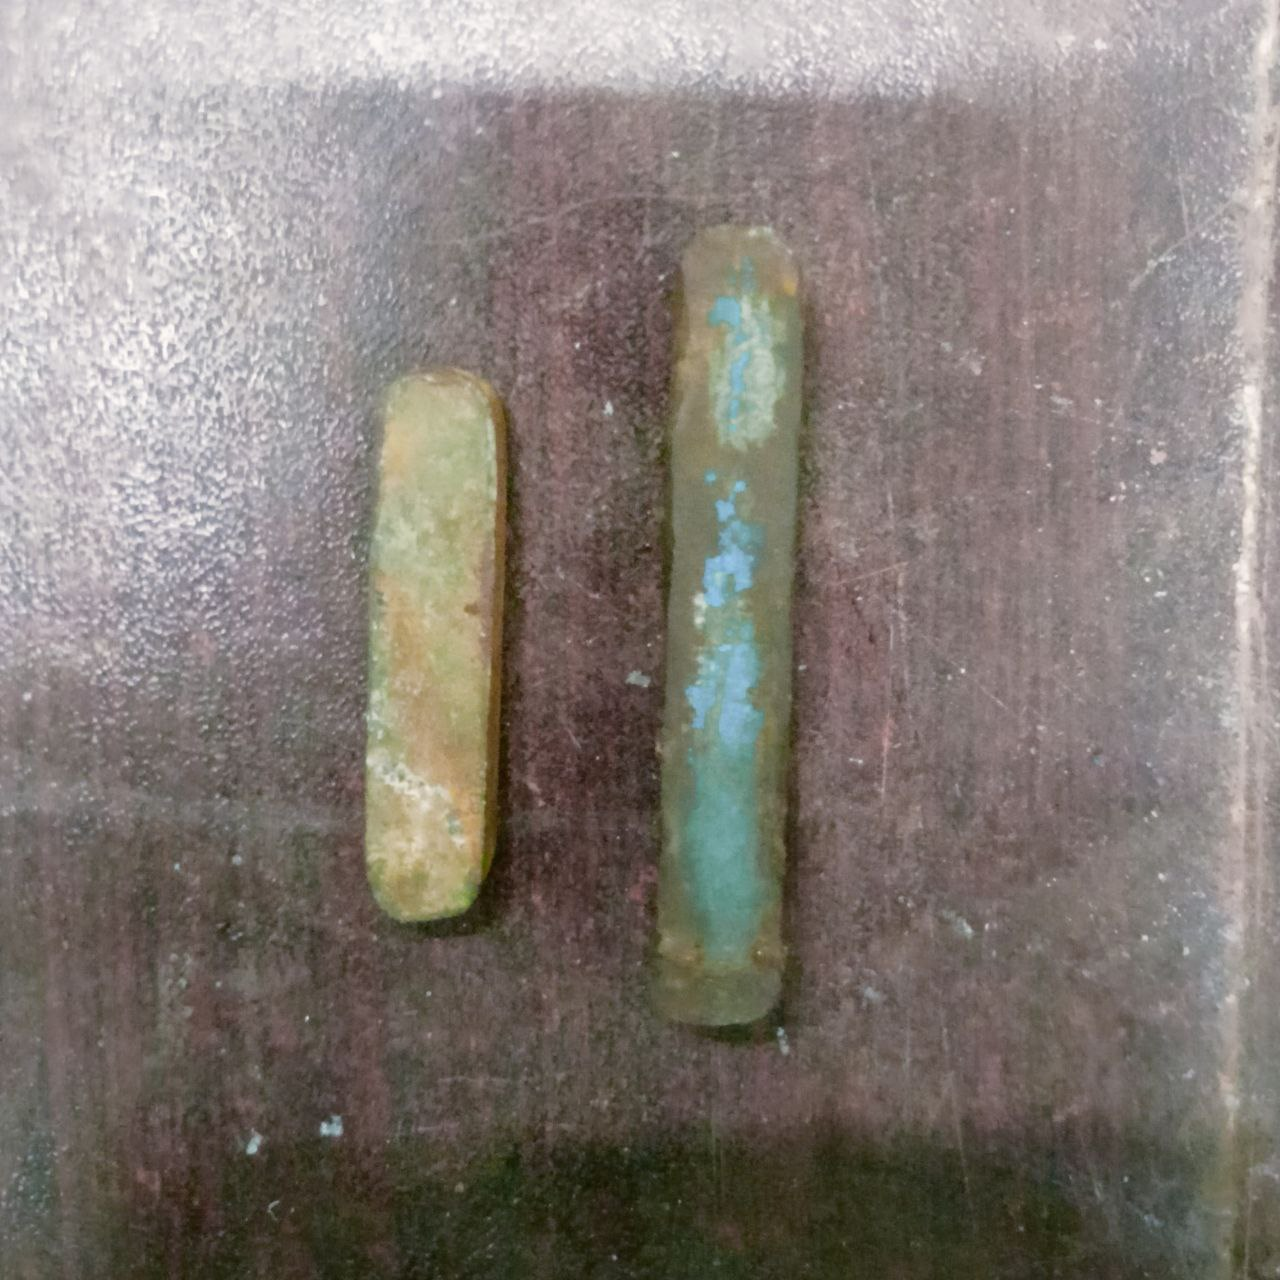
\includegraphics[width=\linewidth]{img/p_08.jpg}
      \caption{Key}
  \end{subfigure}
  \hfill
  \begin{subfigure}{0.3\textwidth}
      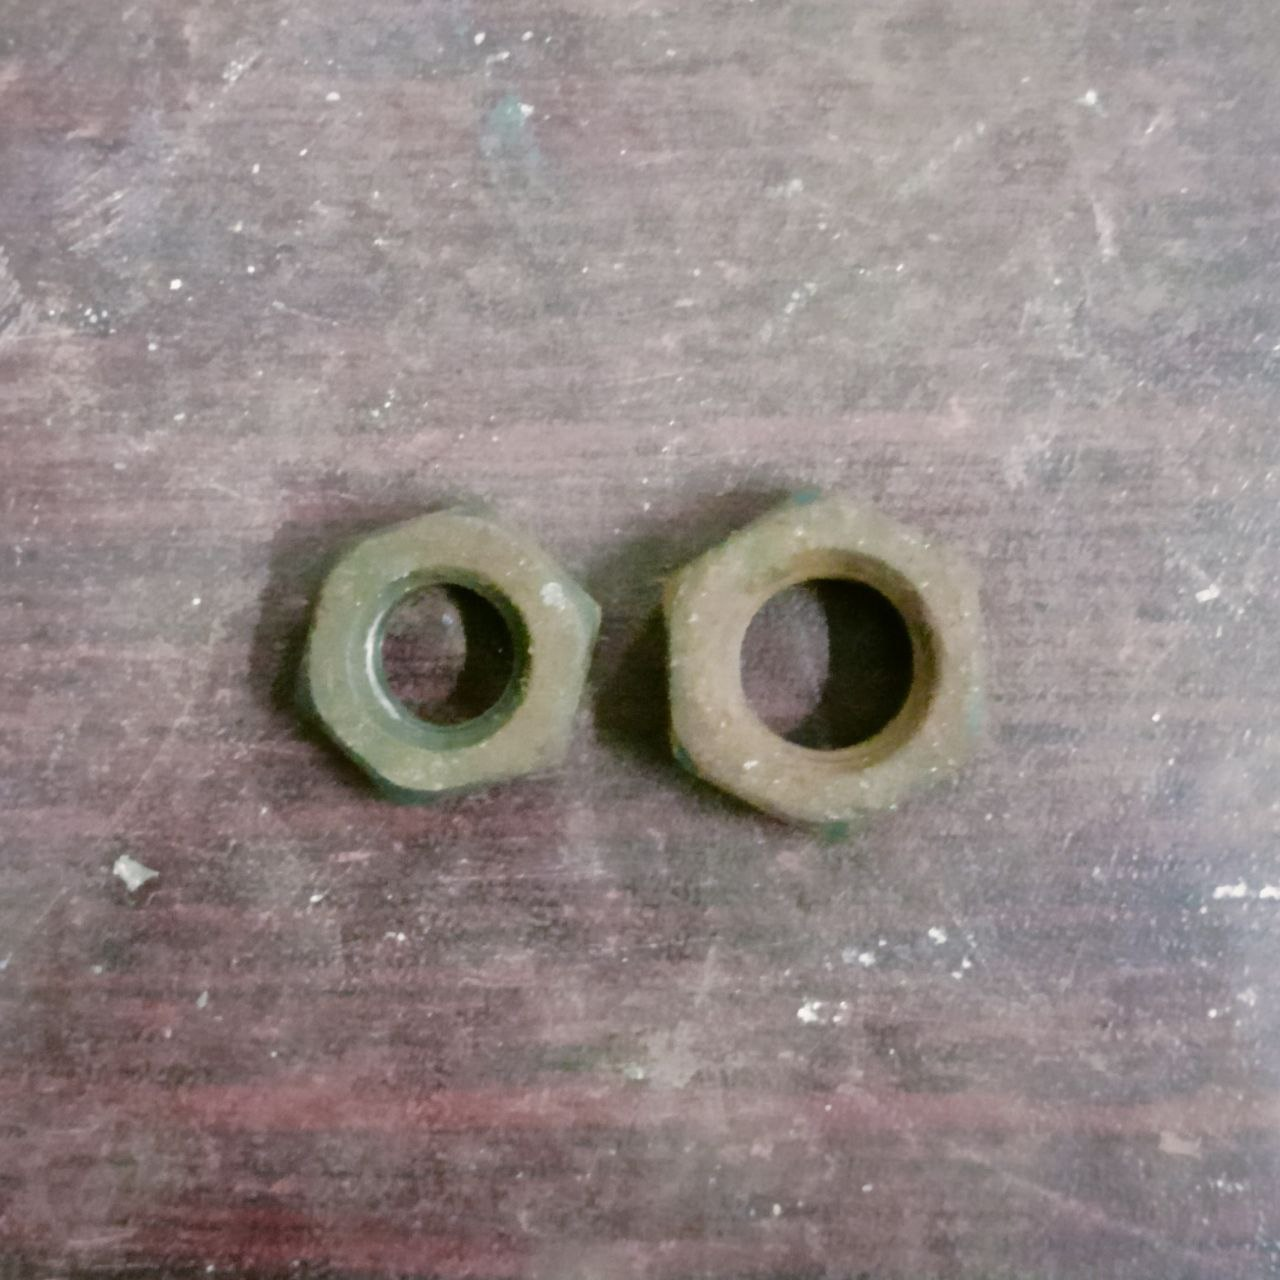
\includegraphics[width=\linewidth]{img/p_09.jpg}
      \caption{Bolts}
  \end{subfigure}

  \caption{Components of Centrifugal Pump}
\end{figure}

 
\subsection*{Components of Centrifugal Pump:}
\begin{itemize}
  \item \textbf{Motor or Driver:} The motor or driver provides the power to rotate the pump's shaft and impeller, enabling the pump to function.
  
  \item \textbf{Impeller:} The impeller accelerates the fluid, increasing its kinetic energy and generating centrifugal force, which helps in moving the fluid through the pump.
  \item \textbf{Casing or Housing:} The casing guides the flow of fluid and converts the kinetic energy imparted by the impeller into pressure energy.
  \item \textbf{Vanes or Diffuser} Increases pressure and reduces velocity of the fluid.
  
  \item \textbf{Wear Rings:} Minimize clearance between impeller and casing, improving efficiency and preventing leakage.
  \item \textbf{Gaskets:} Create tight seals between pump components, preventing fluid leakage.
  
  \item \textbf{Shaft:} The shaft transmits the rotational motion from the motor or driver to the impeller, enabling the pump to operate.
  
  \item \textbf{Bearings:} Bearings support the shaft, reducing friction and allowing smooth rotation. They help maintain the stability and reliability of the pump.
  
  \item \textbf{Seal:} The seal prevents fluid leakage along the shaft, ensuring the integrity of the pump and preventing contamination or loss of fluid.
  
\end{itemize}

\end{document}